%2
\chapter{Phonology: a brief overview}
%\hypertarget{RefHeading18681935131865}

\section{Phonemes}
\label{sec:2:1}
%\hypertarget{RefHeading18701935131865}

The phonological system in Mauwake is quite regular and straightforward, even if not one of the very simplest found in Papuan languages \citep[48--64]{Foley1986}. It has 14 consonants and 5 vowels in its phoneme inventory.  Allophonic variation in Mauwake is very limited, and there is not much morphophonological complexity (\sectref{sec:2.3.3}) either.  In the presentation of the phonology \textsc{ipa} standard phonetic symbols are used.


\subsection{Consonants}
%\hypertarget{RefHeading18721935131865}

The fourteen consonant phonemes in Mauwake are presented in \tabref{tab:2:consonantphonemes}.  \citet[51]{ZGraggen1971} also lists the velar nasal /{\ng}/ as a phoneme in Mauwake, but at least synchronically it is not part of the basic inventory.  All the words in Mauwake that have the velar nasal are shared with a neighbouring language, so they are likely to be borrowings. For those words there is also a native synonym, although it may not be as frequently used. It is also possible that Mauwake has earlier had the velar nasal, as it is a very common areal feature in the Madang North Coast area \citep{ZGraggen1971}. 

\begin{table} 
\caption{Consonant phonemes}
\label{tab:2:consonantphonemes}
\begin{tabular}{lllll}
\mytoprule
 & Bilabial & Alveolar & Palatal & Velar\\
\midrule
Plosive & p  b & t  d &  & k  g\\
Nasal & m & n &  & \\
Fricative & {\textphi} & s &  & \\
Trill &  & r &  & \\
Lateral &  & l &  & \\
Approximant & w &  & j & \\
\mybottomrule
\end{tabular}
\end{table}


Most of the consonant phonemes in Mauwake have only one extrinsic allophone. 

The voiceless \textstyleEmphasizedWords{{plosives}} are unaspirated in all the word positions where they occur \REF{ex:2:voicelessplosives}. They contrast as to bilabial, alveolar and velar points of articulation. Mauwake does not have the glottal stop typical of many Papuan languages. 
\renewcommand{\exfont}{\upshape}
\renewcommand{\eachwordone}{\upshape}
\ea
\label{ex:2:voicelessplosives}
\ea
/{paanek}/  [\textipa{ˈpaːnek}]  `it crashed'
\ex
/{taanek}/  [\textipa{ˈtaːnek}]  `it is full'
\ex
/{kaanek}({e})/  [\textipa{ˈkaːnek(e)}]  `where?'
\ex
/{opa}/  [\textipa{oˈpa}]  `hold!'
\ex
/{otal}/  [\textipa{oˈtal}]  `reef'
\ex
/{oka}/  [\textipa{oˈka}]  `hand drum'
\ex
/{orop}/  [\textipa{oˈrop}]  `descend.\textsc{ss.seq}'
\ex
/{rotorot}/  [\textipa{roˈtorot}]  `painted moray eel'
\ex
/{orok}/  [\textipa{oˈrok}]  `(s)he descended'
\z
\z


The voiceless plosives occur word-initially, -medially and -finally \REF{ex:2:positionofvoicelessplosives}.

\ea\label{ex:2:positionofvoicelessplosives}
\ea
/{pepek}/    [\textipa{peˈpek}]    `enough'\\
\ex
/{onap}/    [\textipa{oˈnap}]    `do.\textsc{ss.seq}'\\
\ex
/{teteke}/   [\textipa{teˈteke}]    `take apart!'\\
\ex
/{menat}/    [\textipa{meˈnat}]    `tide'\\
\ex
/{koka}/    [\textipa{koˈka}]   `bush, jungle'\\
\ex
/{onak}/    [\textipa{oˈnak}]   `his/her mother' \\
\z
\z

The voiced plosives only occur word-initially or medially \REF{tab:2:voicedplosives}. Besides this distributional restriction, their frequency is also markedly lower than that of voiceless plosives. They are not utilized in the derivational or inflectional morphology, except in reduplication. There is voicing harmony affecting the plosives only: when the first two syllables begin with plosives, both of them are either voiced or voiceless. 


\ea
\label{tab:2:voicedplosives}
\ea
/bebeta/  [\textipa{beˈbeta}]  `thin'
\ex
/pepena/  [\textipa{peˈpena}]  `strange'
\ex
/duduwa/  [\textipa{duˈduwa}]  `blunt'
\ex
/tutupila/  [\textipa{tuˈtupila}]  `tadpole'
\ex
/googok/  [\textipa{ˈgoːgok}]  `trevally'
\ex
/kookalija/  [\textipa{ˈkoːkalija}]  `he/she likes'
\ex
/boga/  [\textipa{boˈga}]  `barren, empty (land)'
\ex
/poka/  [\textipa{poˈka}]  `sit down!'
\ex
/dabela/  [\textipa{daˈbela}]  `cold'
\ex
/tapaka/  [\textipa{taˈpaka}]  `cake'
\ex
/gubagel/  [\textipa{guˈbagel}]  `lizard sp.' 
\ex
/kupakup/  [\textipa{kuˈpakup}]  `sago container'
\z
\z

The only exceptions to the voicing harmony are a few words starting with /k/, for instance \REF{ex:2:voicingharmonyexceptions}:

\newpage
\ea
\label{ex:2:voicingharmonyexceptions}
\ea
/kadilam/  [\textipa{kaˈdilam}]  `leech'
\ex
/kibol/  [\textipa{kiˈbol}]  `stinging anemone'
\ex
/kuben/  [\textipa{kuˈben}]  `prawn trap'
\z
\z

The two \textstyleEmphasizedWords{{nasals}} occur word-initially, medially and finally, and contrast as to bilabial and alveolar points of articulation \REF{ex:2:nasals}. 

\ea
\label{ex:2:nasals}
\ea
/manar/  [\textipa{maˈnar}]  `forehead decoration'
\ex
/nanar/  [\textipa{naˈnar}]  `story'
\ex
/moma/  [\textipa{moˈma}]  `taro'
\ex
/mona/  [\textipa{moˈna}]  `fruit species'
\ex
/onam/  [\textipa{oˈnam}]  `I did'
\ex
/onan/  [\textipa{oˈnan}]  `you did'
\z
\z

The \textstyleEmphasizedWords{{fricatives}} contrast as to bilabial/labio-dental and alveolar points of articulation \REF{ex:2:fricatives}. They are both voiceless. The voiceless bilabial fricative /{\textphi}/ [\textipa{\textphi}] occurs word-initially and medially, the alveolar grooved fricative /s/ [s] occurs word-initially, -medially and \nobreakdash-finally. 

\ea
\label{ex:2:fricatives}
\ea
/{\textphi}ariar-/  [\textipa{{\textphi}aˈriar}-]  `abstain'
\ex
/sariar-/  [\textipa{saˈriar}-]  `get well'
\ex
/kosija/  [\textipa{koˈsija}]  `it comes out of mouth'
\ex
/ko{\textphi}ija/  [\textipa{koˈ{\textphi}ija}]  `he hammers'
\ex
/kawus/  [\textipa{kaˈwus}]  `smoke'
\z
\z

A possible reason for the restricted distribution of /{\textphi}/ is that it is a result of a sound change, which is discussed at the end of the consonant section.

The voiced alveolar \textstyleEmphasizedWords{{trill}} /r/ [r] occurs in free variation with the voiced alveolar flap [{\textfishhookr}] word-initially, -medially and -finally \REF{ex:2:trill}.  

\ea
\label{ex:2:trill}
\ea 
/rowirow/  [\textipa{roˈwirow}] {\Tilde} [\textipa{{\textfishhookr}o{ˈwi}{\textfishhookr}ow}]  `giant clam'
\ex
/ewar/  [\textipa{eˈvar}] {\Tilde} [\textipa{eˈva{\textfishhookr}}]  `west wind'
\z
\z

The voiced alveolar \textstyleEmphasizedWords{{lateral}} /l/ [l] occurs word-initially, -medially and -finally \REF{ex:2:lateral}. 

\ea
\label{ex:2:lateral}
\ea
/lali/  [\textipa{laˈli} ]  `small reef fish'
\ex
/kaul/  [\textipa{ˈkaul}]  `hook'
\z
\z

In many Papuan languages [l] and [r] are allophones of the same phoneme, but in Mauwake they are separate phonemes, contrasting with each other \REF{ex:2:lrcontrast}:
\newpage

\ea
\label{ex:2:lrcontrast}
\ea
/liilin-/  [\textipa{liːlin-}]  `sting, smart (v.)'
\ex
/riirin-/  [\textipa{ˈriːrin}] {\Tilde} [\textipa{ˈ{\textfishhookr}iː{\textfishhookr}in-}]  `quarrel (v.)'
\ex
/kalan-/  [\textipa{kaˈlan}-]  `have nausea' 
\ex
/karan-/  [\textipa{kaˈran}] {\Tilde} [\textipa{kaˈ{\textfishhookr}an-}]  `shake'
\ex
/nanal/  [\textipa{naˈnal}]  `tree sp.'
\ex
/nanar/  [\textipa{naˈnar}]  `story'
\z
\z

Yet in a few words the two fluctuate \REF{ex:2:lrfluct}. This seems to be a dialectal difference.

\ea
\label{ex:2:lrfluct}
\ea
/eliwa/  [\textipa{eˈliva}] {\Tilde} [\textipa{eˈriva}]  `good'
\ex
/saliwija/  [\textipa{saˈlivija}] {\Tilde} [\textipa{saˈrivija}]  `(s)he heals/repairs'
\z
\z 

There are two approximants, or \textstyleEmphasizedWords{{semivowels}}: [w] and [j].  They are interpreted as consonants when occurring in syllable onset or coda, and as vowels when forming part of the syllable nucleus. 

The alveo-palatal semivowel /j/ [j] occurs word-initially and -medially. The voiced alveo-palatal grooved fricative [{\textyogh}] is used instead of [j] in the inland (Papur) and Ulingan dialects \REF{ex:2:semiVj}.

\ea
\label{ex:2:semiVj}
\ea
/jakiya/  [\textipa{jaˈkija}] {\Tilde} [\textipa{{\textyogh}a{ˈki}{\textyogh}a}]  `(s)he bathes'
\ex
/jaisow/  [\textipa{ˈjaisow} ] {\Tilde} [\textipa{ˈ{\textyogh}aisow}]  `I alone' 
\z
\z

The bilabial semivowel /w/ has the following allophones \REF{ex:2:semiVw}:

\begin{itemize}
 \item{} [w]  \textstyleListBaseChar{the voiced bilabial semivowel occurs next to a rounded vowel, fluctuating with [v] when between a preceding unrounded and a following rounded vowel};
 \item{} [v]  the voiced labio-dental frictionless continuant occurs elsewhere;
 \item{} [β]  the voiced bilabial fricative occurs fluctuating with both [w] and [v] in the inland (Papur) dialect, very strongly in the village of Yeipamir.
\end{itemize}


\ea 
\label{ex:2:semiVw}
\ea
/wowosa/  [\textipa{woˈwosa}] {\Tilde} [\textipa{βoˈβosa}]  `bud'
\ex
/now/  [\textipa{now}] {\Tilde} [\textipa{noβ}]  `stonefish'
\ex
/kuwiwi/  [\textipa{kuˈwiwi}] {\Tilde} [\textipa{kuˈβiβi}]  `blue-lined surgeonfish'
\ex
/iwoka/  [\textipa{iˈwoka}]{\Tilde}[\textipa{iˈvoka}]{\Tilde}[\textipa{iˈβoka}]  `yam'
\ex
/iwera/  [\textipa{iˈvera}] {\Tilde} [\textipa{iˈβera}]  `coconut'
\ex
/elew/  [\textipa{eˈlev}] {\Tilde} [\textipa{eˈleβ}]\footnote{All these different optional allophonic variations of /w/ are not listed in the phonetic representations below, unless relevant to the discussion in the main text of the section. The same applies to the variation of /{\textphi}/, /r/ and /j/.}  `in-law'
\z
\z


The reasons for analyzing the semivowels as consonants are as follows:


\begin{itemize}
\item There are no unambiguous 3-vowel sequences word-initially; 
\item Both the semivowels have a fricative allophone;
\item There are no unambiguous glides starting with a mid vowel; 
\item The geminate non-high vowels only occur in initial syllables;
\item If they were interpreted as vowels, the stress pattern of some words would not follow the otherwise exceptionless stress placement rule.
\end{itemize}

\ea
\ea
/wiwisa/  [\textipa{viˈvisa}] {\Tilde} [\textipa{βiˈβisa}]  `murky'
\ex
/jaisow/  [\textipa{ˈjaisow}] {\Tilde} [\textipa{ˈ{\textyogh}aisow}]  `I alone'
\ex
/marew/  [\textipa{maˈrev}] {\Tilde} [\textipa{maˈreβ}]  `none'
\ex
/now/  [\textipa{now}] {\Tilde} [\textipa{noβ}]  `stonefish'
\ex
/jakijem/  [\textipa{jaˈkijem}] {\Tilde} [\textipa{{\textyogh}aˈki{\textyogh}em}]  `I bathe'
\ex
/uruwa/  [\textipa{uˈruwa}] {\Tilde} [\textipa{uˈruβa}]  `loincloth'
\z
\z

The following sets of examples show clear contrasts between the semivowel /w/ and the vowel /u/, and between the semivowel /j/ and the vowel /i/ \REF{ex:2:semiV-contrasts}:

\ea 
\label{ex:2:semiV-contrasts}
\ea
/wulinija/  [\textipa{wuˈlinija}]  `it shines'
\ex
/uusakija/  [\textipa{ˈuːsakija}]  `he/she roasts'
\ex
/wuunija/  [\textipa{ˈwuːnija}]  `(wind) blows'
\ex
/uuwunija/  [\textipa{ˈuːwunija}]  `(s)he talks'
\ex
/wuwusirap  [\textipa{wuˈwusirap}]  `name of a month'
\ex
/lalu/  [\textipa{laˈlu}]  `parrotfish'
\ex
/diluw/  [\textipa{diˈluw}] {\Tilde} [\textipa{diˈluβ}]  `vine sp.'
\ex
/jena/  [\textipa{jeˈna}] {\Tilde} [\textipa{{\textyogh}eˈna}]  `my'
\ex
/jiena/  [\textipa{jiˈena}] {\Tilde} [\textipa{{\textyogh}iˈena}]  `our'
\ex
/iina/  [\textipa{ˈiːna}]  `mosquito'
\ex
/jiija/  [\textipa{ˈjiːja}] {\Tilde} [\textipa{ˈ{\textyogh}iː{\textyogh}a}]  `(s)he gives to me'
\z
\z

In a few words a semivowel is adjacent to a homorganic vowel, but such a contrast as above is not available, and the regular syllable patterns and the stress placement rule allow for two or more interpretations. Also, the pronunciation varies slightly from village to village and between individuals.  In these cases the decision how to represent the word phonemically is somewhat arbitrary \REF{ex:2:semiV-ambig}.

\ea
\label{ex:2:semiV-ambig}
\ea
/jaamun/  [\textipa{ˈjaːmun}] {\Tilde} [\textipa{j{\textsci}ˈamun}]  `my/our younger sibling'
\ex
/jaaja/  [\textipa{ˈjaːja}] {\Tilde} [\textipa{ˈjaija}]  `my/our maternal uncle'
\ex
/waaja/  [\textipa{ˈwaːja}] {\Tilde} [\textipa{ˈwaija}] {\Tilde} [\textipa{ˈwuaija}]  `pig'
\ex
/wuija/  [\textipa{ˈwuija}] {\Tilde} [\textipa{ˈwaija}] {\Tilde} [\textipa{ˈwuaija}]  `(s)he puts'
\z
\z

The \textstyleEmphasizedWords{{bilabial}} consonants contrast word-initially and -medially; those consonants that can occur word-finally contrast in this position too \REF{ex:2:bilabCons}. 

\ea
\label{ex:2:bilabCons}
\ea
/poka/  [\textipa{poˈka}]  `house post'
\ex
/boga/  [\textipa{boˈga}]  `empty, barren (land)'
\ex
/moma/  [\textipa{moˈma}]  `taro'
\ex
/\textipa{{\textphi}oma}/  [\textipa{{\textphi}oˈma}]  `ashes'
\ex
/womar/  [\textipa{woˈmar}]  `his cousin'
\ex
/epa/  [\textipa{eˈpa}]  `place'
\ex
/bebaura/  [\textipa{beˈbaura}]  `tree sp.'
\ex
/ema/  [\textipa{eˈma}]  `mountain'
\ex
/e{\textphi}a/  [\textipa{eˈ{\textphi}a}]  `me'
\ex
/ewar/  [\textipa{eˈvar}]  `west wind'
\ex
/orop/  [\textipa{oˈrop}]  `descend.\textsc{ss.seq}'
\ex
/orom/  [\textipa{oˈrom}]  `I descended'
\ex
/arow/  [\textipa{aˈrow}]  `three'
\z
\z


The \textstyleEmphasizedWords{{alveolar}} consonants contrast in word-initial and -medial positions, and those that can occur in word-final position contrast in that position as well \REF{ex:2:alveolarCons}.

\ea
\label{ex:2:alveolarCons}
\ea
/tawowola/  [\textipa{taˈwowola}]  `rubbish'
\ex
/dabela/  [\textipa{daˈbela}]  `cold'
\ex
/nabena/  [\textipa{naˈbena}]  `carrying pole'
\ex
/sawur/  [\textipa{saˈwur}]  `spirit'    
\ex
/raapa/  [\textipa{ˈraːpa}]  `bag'
\ex
/labuela/  [\textipa{laˈbuela}]  `pawpaw'
\ex
/otal/  [\textipa{oˈtal}]  `reef'
\ex
/odaweleka/  [\textipa{oˈdaweleka}]  `gill'
\ex
/onam/  [\textipa{oˈnam}]  `I did'
\ex
/osaiwa/  [\textipa{oˈsaiva}]  `bird of paradise'
\ex
/oraija/  [\textipa{oˈraija}]  `he/she descends'
\ex
/olal/  [\textipa{oˈlal}]  `fish species'
\ex
/menat/  [\textipa{meˈnat}]  `tide'
\ex
/konan/  [\textipa{koˈnan}]  `garfish'
\ex
/oras/  [\textipa{oˈras}]  `spinefoot (fish)'
\ex
/nanar/  [\textipa{naˈnar}]  `story'
\ex
/nanal/  [\textipa{naˈnal}]  `tree sp.'
\z
\z

The \textstyleEmphasizedWords{{velar}} and \textstyleEmphasizedWords{{alveo-palatal}} consonants contrast word-initially and -medially \REF{ex:2:velarCons}. Word-finally /j/ does not occur at all, and /g/ is extremely rare.\footnote{There are only 4 occurrences of word-final /g/ in the lexicon of over 3600 words. Those may all be loans from neighbouring languages.}

\ea
\label{ex:2:velarCons}
\ea
/kia/  [\textipa{k\textsci{ˈ}a}]  `white'
\ex
/gia/  [\textipa{g\textsci{ˈ}a}]  `baby'
\ex
/jia/  [\textipa{j\textsci{ˈ}a}]  `us'
\ex
/magok/  [\textipa{maˈgok}]  `woven band'
\ex
/makak/  [\textipa{maˈkak}]  `brown quail'
\ex
/majona/  [\textipa{maˈjona}]  `brown-collared bush turkey'
\z
\z

Both the distributional restrictions of some consonant phonemes and some regular sound correspondences between Mauwake and the related Kaukombaran languages\linebreak point to earlier sound changes. My tentative suggestion is that the voiced plosives /b/ and /g/\footnote{There are too few words with /d/ and /t/ in the sample to make a meaningful comparison, and what data is available does not indicate that they participated in the change.}  in Mauwake became devoiced at some earlier stage, and the present-day voiced plosives are a later development. In the Kaukombaran languages voiced plosives are much more frequent than in Mauwake, and there is a clear sound correspondence between many cognates.\footnote{The Kaukombaran data is from \citet{LoewekeEtAl1982} and \citep{ZGraggen1980}.} \tabref{tab:2:plosivesoundcorrespondences} lists seven cognates in four languages. In the comparison the words are listed in phonetic form but without the brackets; the phonemic representation is basically the same. 

\begin{table}
 \caption{Sound correspondences in plosives}
 \label{tab:2:plosivesoundcorrespondences}
\begin{tabular}{lllll}
\mytoprule
Mauwake  &Miani  &Maia  &Pila\\
\midrule
 paapa &  baba & bab & mbab & `elder sibling'\\
pok-  &bug- & buge- & buge- & `sit'\\
perek- & bereg- & bered- & buroaind- & `tear (v.)'\\
kemena  & kema  &goama & {\ng}goama  & `inside'\\
kukusa  &gugun  &  &gugut  &`shadow, picture'\\
\mybottomrule
\end{tabular}
\end{table} 


I suggest that /{\textphi}/ in Mauwake is a result of a sound change whereby /w/ in certain positions became devoiced and changed into a fricative. This can be seen in the sound correspondences in cognate words in related Kaukombaran languages \tabref{tab:2:fricativesoundcorrespondences}.\footnote{Note that within the Kaukombaran group there has also been change from /w/ into /b/.  Another possibility is that /b/ has first changed into /w/ and further into /{\textphi}/ in Mauwake, but that seems less likely because there are numerous other words with /b/ which do not participate in this sound change.}

\clearpage
\begin{table}
\caption{Sound correspondences in bilabial continuants}
\label{tab:2:fricativesoundcorrespondences}
\begin{tabular}{lllll}
\mytoprule
Mauwake  &Miani  &Maia  &Pila\\
\midrule
a{\textphi}ila & abir&  koawir & kuawir & `grease' \\
a{\textphi}ura & ab & kab&  kap & `lime'\\
i{\textphi}era&  ibor & ibor&  iwor & `sea'\\
uru{\textphi}- & ruw- & uruw- & &   `see'\\
{\textphi}ar- & bar- & war- & &  `call'\\
u{\textphi}-   & uw- & ube- & waguwa-  & `dance'\\
\mybottomrule 
\end{tabular}
\end{table}

\subsection{Vowels}
%%\hypertarget{RefHeading18741935131865}


There is variation in the Papuan languages from the 3-vowel systems in Ndu languages to an 8-vowel system in Vanimo. The basic and a very common one is a 5-vowel system \citep[49--54]{Foley1986}, also the most common worldwide \citep[126]{Maddieson1984}.  It is employed by Mauwake as well, and the vowels are the ones that \citet[125]{Maddieson1984} lists as the most common vowels universally (\tabref{tab:3:vowelphonemes}). 
 
\begin{table}
\caption{Vowel phonemes}
\label{tab:3:vowelphonemes}
\begin{tabular}{llll}
\mytoprule
& Front & Central & Back\\
\midrule
High & i &  & u\\
Mid & e &  & o\\
Low &  & a & \\
\mybottomrule
\end{tabular}
\end{table}


The five vowel phonemes are voiced and oral. They contrast as to front, central and back points of articulation. Front and back vowels also have a high vs. mid contrast. There is only one set of mid vowels in Mauwake, which are phonetically between the \textsc{ipa} higher and lower mid vowels.  For the sake of simplicity, I have represented them with the \textsc{ipa} symbols for higher mid vowels, /e/ and /o/.\footnote{To distinguish the true mid vowels from higher mid vowels \citet[123]{Maddieson1984} writes them with quote marks: ``e'' and ``o''.}  Both the front vowels are unrounded and the back vowels rounded.

The mid vowels could also be analyzed as non-high vowels together with the low central vowel /a/, thus simplifying the chart, since there are no front or back low vowels. That grouping \textstyleEmphasizedWords{is} actually used in \sectref{sec:2.3.3}, where it simplifies the past tense suffix rule. But the distributional fact that there are no vowel glides beginning with either /e/ or /o/ justifies distinguishing them as a separate group of mid vowels.  

The high vowels /i/ and /u/ have an open allophone, [{\textsci}] and [{\textupsilon}] respectively, following a word-initial consonant and preceding a central vowel /a/ (Rule \ref{ex:2:vowelrule}). In other positions they have a more closed allophone [i] and [u] \REF{ex:2:highvowelallophones}. The other vowels do not have allophonic variation.

\ea
\label{ex:2:vowelrule}
\begin{tabular}{c}V\\+high\\+close\end{tabular}
\begin{tabular}{c}$\to$\\~\\~\end{tabular}
\begin{tabular}{c}V\\+high\\+open\end{tabular}
\begin{tabular}{c}/\_\_\\~\\~\end{tabular}
\begin{tabular}{c}V\\+central\\~\end{tabular}
\z

\ea
\label{ex:2:highvowelallophones}
\ea
/ikina/  [\textipa{iˈkina}]  `smell'
\ex
/lali/  [\textipa{laˈli}]  `small fish'
\ex
/mia/  [\textipa{m{\textsci}ˈa}]  `body'
\ex
/uruwa/  [\textipa{uˈruwa}]  `loincloth'
\ex
/lalu/  [\textipa{laˈlu}]  `parrotfish'
\ex
/mua/  [\textipa{m{\textupsilon}ˈa}]  `man'
\z
\z

The vowels contrast word-initially, -medially and -finally \REF{ex:2:vowelcontrasts}:

\ea
\label{ex:2:vowelcontrasts}
\ea
/a{\textphi}a/  [\textipa{aˈ{\textphi}a}]  `flying fox'
\ex
/e{\textphi}a/  [\textipa{eˈ{\textphi}a}]  `me'
\ex
/i{\textphi}a/  [\textipa{iˈ{\textphi}a}]  `snake'
\ex
/o{\textphi}a/  [\textipa{oˈ{\textphi}a}]  `colour'
\ex
/u{\textphi}a/  [\textipa{uˈ{\textphi}a}]  `swing (n.)'
\ex
/marari/  [\textipa{maˈrari}]  `temporary (shelter)'
\ex
/maremuka/  [\textipa{maˈremuka}]  `corn (med.)'
\ex
/marija/  [\textipa{maˈrija}]  `(s)he scrapes'
\ex
/maroka/  [\textipa{maˈroka}]  `prawn'
\ex
/saruwa/  [\textipa{saˈruwa}]  `tree sp.'
\ex
/popoka/  [\textipa{poˈpoka}]  `unripe fruit'
\ex
/ooke/  [\textipa{ˈoːke}]  `follow him!'
\ex
/loloki/  [\textipa{loˈloki}]  `plant sp.'
\ex
/papako/  [\textipa{paˈpako}]  `some'
\ex
/ooku/  [\textipa{ˈoːku}]  `let's (dual) follow him!'
\z
\z

Phonemic vowel length only occurs in word-initial syllables.  Long vowels are interpreted as two vowels of the same quality for the following reasons:


\begin{itemize}
\item Other vowel sequences are common in Mauwake;
\item The quality of the long and short vowel is the same;
\item Economy of description: there are five vowels instead of ten.
\end{itemize}

Long and short vowels contrast with each other \REF{ex:2:longshortcontrasts}:

\ea
\label{ex:2:longshortcontrasts}
\ea
/aasa/  [\textipa{ˈaːsa}]  `canoe'
\ex
/asa/  [\textipa{aˈsa}]  `wild \textstyleForeignWords{galip} nut'
\ex
/peela/  [\textipa{ˈpeːla}]  `rotten'
\ex
/pela/  [\textipa{peˈla}]  `leaf'
\ex
/kiira/  [\textipa{ˈkiːr}a]  `side, shin'
\ex
/kira/  [\textipa{kiˈra}]  `wild sugarcane'
\ex
/{\textphi}uura/  [\textipa{ˈ{\textphi}uːra}]  `steep'
\ex
/{\textphi}ura/  [\textipa{{\textphi}uˈra}]  `knife'
\z
\z

\subsection{Suprasegmentals: stress and intonation}
%%\hypertarget{RefHeading18761935131865}


Since Mauwake is not a tonal language, the only suprasegmentals discussed here are stress and intonation.

\subsubsection{Stress}\label{sec:2.1.3.1}
%%\hypertarget{RefHeading18781935131865}


Stress is not phonemic in Mauwake, but three degrees of phonetic stress are discernible in a word.  Primary stress is marked by greater intensity, higher fundamental frequency and often, but not always, by non-phonemic lengthening of the vowel.  An unstressed syllable is considerably weaker, but the vowels still retain their essential quality.  A syllable with a secondary stress is weaker than one with primary stress, but stronger than an unstressed syllable. Since stress is a defining factor on the word level, it is discussed further in \sectref{sec:2.3}.

Stress has a pragmatic function on clause and sentence level. The clausal stress manifests itself in slightly greater loudness and intensity than that of the ordinary word stress, and its default position is the verb or the non-verbal predicate. In a multi-clause sentence the final verb typically receives the strongest clausal stress; this may be called sentence stress if it needs to be distinguished from the clausal stress of the non-final clauses. The position of the clausal stress may be shifted to give added prominence to some element in the clause (\sectref{sec:9.2.3}). When this is done, the loudness and intensity of the stressed syllable are increased, and non-phonemic lengthening of the vowel may take place.

\subsubsection{Intonation}\label{sec:2.1.3.2}
%%\hypertarget{RefHeading18801935131865}


The three grammatical units important from the point of view of intonation are a phrase, a (non-final) clause and a sentence. All final clauses are here treated as sentences.

Pitch variations in Mauwake are not very prominent, and in general the register is quite low compared e.g. with English. There is more register variation in the inland than on the coast. 

The most common sentence intonation contour is falling. The first stressed syllable is the highest; after it the intonation falls very gradually until the word with the sentence stress, typically the final verb. There is a slight rise at the syllable with the sentence stress, and then a very sharp fall in the terminal contour.  This same basic pattern occurs both in statements \REF{ex:2:x898}, commands \REF{ex:2:x1769}, in non-polar questions \REF{ex:2:x899} and certain polar questions \REF{ex:2:x902}. In the following examples, the word with the sentence stress is bolded.


\xbox{\textwidth}{
\ea%x898
\label{ex:2:x898}
% 
\includegraphics[width=\textwidth]{figures_mod/image8.jpeg}
\gll [\linieb{20}{jo} 
\linieb{18}{mo}\linieb{20}{ˈma}
\textstyleEmphasizedVernacularWords{
\linieb{14}{e}\linieb{16}{ˈni-}\dline{16}{3}{26}m-i-jem}] \\ 
I  taro  eat-\textsc{nps}-\textsc{pr}.1s     \\
\glt`I (am) eat(ing) taro.'
\z
}


In commands the intonation contour is very much the same as in a statement, but the pronunciation is phonetically more tense.

\xbox{\textwidth}{
\ea%x1769
\label{ex:2:x1769}
% 
\includegraphics[width=\textwidth]{figures_mod/image9.jpeg}
\gll [\linieb{16}{mo}\linieb{20}{ˈma}
\textstyleEmphasizedVernacularWords{
\linieb{14}{e}ˈ\linieb{16}{ni}\dline{16}{2}{18}m-eka}] \\
taro  eat-\textsc{imp}.2p      \\
\glt`Eat (\textsc{pl}) taro!'
\z
}

In non-polar questions the sentence-final intonation is also falling. The stressed syllable of the question word carries the sentence stress if it is emphasized \REF{ex:2:x901}, but often there is only a slightly higher rise than there would be in other words in the same position, and the sentence stress is placed on the stressed syllable of the final verb \REF{ex:2:x899}, \REF{ex:2:x900}.



\xbox{\textwidth}{
\ea%x901
\label{ex:2:x901}
% 
\includegraphics[width=\textwidth]{figures_mod/image10.jpeg}
\gll [%
\linieb{24}{ˈmuː}\linieb{20}{ka}
\linieb{22}{ˈnain}
\textstyleEmphasizedVernacularWords{
\linieb{16}{mo}%
\linieb{20}{ˈram}
} 
\linieb{12}{o}\linieb{14}{ˈmo}%
\dline{14}{2}{20}m-i-ja] \\
boy  that1  why  cry-\textsc{Np-pr}.3s      \\
\glt`\textit{Why} is that boy crying?'
\z
}



\xbox{\textwidth}{
\ea%x899
\label{ex:2:x899}
% 
\includegraphics[width=\textwidth]{figures_mod/image11.jpeg}
\gll%
 [%
\linieb{16}{maː} %
\textstyleEmphasizedVernacularWords{
\linieb{22}{ˈmau}\linieb{18}{wa}
}
\linieb{12}{e}%
\linieb{14}{ˈni}%
\dline{14}{2}{20}m-i-n%
] \\
thing  what  eat-\textsc{Np-pr}.2s      \\
\glt`What are you eating?'
\z
}



\xbox{\textwidth}{
\ea%x900
\label{ex:2:x900}
% 
\includegraphics[width=\textwidth]{figures_mod/image12.jpeg}
\gll%
 [%
\linieb{18}{m{\textupsilon}a}
\textstyleEmphasizedVernacularWords{%
\linieb{22}{ˈnaː}%
\linieb{20}{re}%
\linieb{18}{we}%
\linieb{16}{=ke}
} 
\linieb{12}{e}\linieb{14}{ˈka}%
\dline{14}{2}{16}p-o-k%
] \\
man  who=\textsc{cf}  come-\textsc{pa}-3s      \\
\glt`Who came?'
\z
}

\newpage	
The only instance where there can be any rising intonation sentence-finally is a polar question.  It is only used when the speaker is uncertain whether the answer is going to be affirmative or negative \REF{ex:2:x902}.  The rise is on the question clitic =\textstyleStyleVernacularWordsItalic{i}.  



\xbox{\textwidth}{
\ea%x902
\label{ex:2:x902}
% 
\includegraphics[width=\textwidth]{figures_mod/image13.jpeg}
\gll %
[%
\linieb{20}{ˈau}%
\linieb{18}{wa}
\textstyleEmphasizedVernacularWords{%
\linieb{14}{e}%
\linieb{16}{ˈka}%
\dline{16}{2}{24}%
p-o-k=%
\rise{8}%
i%
}%
]\\
 father  come-\textsc{pa}-3s=\textsc{qm}     \\
\glt`Did father come?'
\z
}

If the speaker strongly expects the answer to agree with the polarity of the question, the intonation is falling \REF{ex:2:x903}. Since polar questions are are also marked with a question marker \textstyleStyleVernacularWordsItalic{=}\textstyleStyleVernacularWordsItalic{i} sentence-finally, a separate intonation pattern is partly redundant.



\xbox{\textwidth}{
\ea%x903
\label{ex:2:x903}
% 
\includegraphics[width=\textwidth]{figures_mod/image14.jpeg}
\gll%
 [%
\linieb{20}{ˈau}%
\linieb{18}{wa}
\textstyleEmphasizedVernacularWords{%
\linieb{14}{e}%
\linieb{16}{ˈka}%
\dline{16}{2}{26}{p-o-k=i}}%
] \\
 father  come-\textsc{pa}-3s=\textsc{qm}     \\ 
\glt`Did father come?' (Expecting ``yes'' as an answer.)
\z
}

The intonation pattern in medial clauses, instead of falling at the end, is either level or slightly rising.  The more expected the sequence, the more level the intonation is. In \REF{ex:2:x904} the two clauses are part of an ``expectancy chain'', because coconuts are scraped only for preparing food. (In the following three examples, the medial and subordinate clauses are bolded rather than the verb of the finite clause.)


 

\xbox{\textwidth}{
\ea%x904
\label{ex:2:x904}
% 
\includegraphics[width=\textwidth]{figures_mod/image15.jpeg}
\gll [\textstyleEmphasizedVernacularWords{%
\linieb{18}{iˈ}%
\linieb{20}{we}%
\linieb{16}{ra}
} %
\textstyleEmphasizedVernacularWords{%
\linieb{14}{mu}%
-\linieb{14}{ˈep}
}  %
\linieb{10}{maa} %
\linieb{12}{ˈuu}%
\dline{12}{3}{24}p-i-nen] \\
coconut  scrape-\textsc{ss.seq} food  cook-\textsc{Np-fu}.1s      \\
\glt`I will scrape a coconut and cook food.'
\z
}

But \REF{ex:2:x905} tells about an unexpected event, a person finding a turtle when he had just gone fishing; instead of catching it he might have either chosen to leave it or failed to catch it.

 

\xbox{\textwidth}{
\ea%x905
\label{ex:2:x905}
% 
\includegraphics[width=\textwidth]{figures_mod/image16.jpeg}
\gll %
[\textstyleEmphasizedVernacularWords{%
\linieb{24}{pon}
} %
\textstyleEmphasizedVernacularWords{
\linieb{20}{u}%
\linieb{22}{ˈru}%
\dline{22}{2}{10}%
{\textphi-}%
\rise{18}ap
} %
\textstyleEmphasizedVernacularWords{\linieb{16}{ˈaː}%
\dline{16}{2}{12}w-%
\rise{12}ep
} %
\linieb{10}{p-e}%
\linieb{12}{ˈka}%
\dline{12}{2}{18}p-e-m] \\
 turtle  see-\textsc{ss.seq}  take-\textsc{ss.seq} \textsc{bpx}-come-\textsc{pa}-1s     \\
\glt`I saw a turtle, caught it and brought it (here).'
\z
}

\largerpage
The rising intonation is more common in subordinate clauses; in conditional clauses \REF{ex:2:x906} it is particularly noticeable.  As a rule, the more important the speaker considers the clause as a presupposition for the main clause, the more clearly there is an intonational rise clause-finally.  



\xbox{\textwidth}{
\ea%x906
\label{ex:2:x906}
% 
\includegraphics[width=\textwidth]{figures_mod/image17.jpeg}
\gll %
[\textstyleEmphasizedVernacularWords{
\linieb{24}{i}%
\linieb{26}{ˈ{\textphi}a}
}
\textstyleEmphasizedVernacularWords{
\linieb{22}{u}%
\linieb{24}{ˈru}%
\linieb{20}{{\textphi}-i}%
\dline{20}{3}{26}-nen=%
\rise{13}{na}} 
\linieb{14}{ke}%
\linieb{16}{ˈker} %
\linieb{10}{o}%
\linieb{12}{ˈp-i}%
\dline{12}{2}{14}-nen]\\
 snake  see-\textsc{Np-fu}.1s=\textsc{tp}  fear  hold-\textsc{nps}-\textsc{fu}.1s\\
\glt`If I see a snake, I will be afraid.'
\z
}

A phrase that is fronted as a left-dislocated theme (\sectref{sec:9.1}) also has a rising intonation at the end of the phrase.  The phrase, bolded in \REF{ex:2:x907}, occurs at the beginning of the clause.  The slash indicates a pause.

 

\xbox{\textwidth}{
\ea%x907
\label{ex:2:x907}
% 
\includegraphics[width=\textwidth]{figures_mod/image18.jpeg}
\gll %
[\textstyleEmphasizedVernacularWords{%
\linieb{28}{ˈjos}%
\linieb{24}{=n}%
\rise{26}a
%
}/
\linieb{20}{ o}%
\linieb{24}{ˈwow} %
\linieb{18}{ma}%
\linieb{20}{ˈne}%
\linieb{16}{ka}
\linieb{14}{me}
\linieb{10}{i}%
\linieb{12}{ˈki}%
\linieb{10}{w-i}%
\dline{10}{3}{16}-jem] \\
1s.\textsc{fc}=\textsc{tp}  village  big  not  go-\textsc{Np-}\textsc{pr}.1s      \\
\glt`As for me, I don't go to town.'
\z
}
  
In listing, the intonation rises very slightly at the final syllable of each non-final phrase listed, or is retained at the same level as the previous syllable(s) \REF{ex:2:x908}.


 
\xbox{\textwidth}{
\ea%x908
\label{ex:2:x908}
% 
\includegraphics[width=\textwidth]{figures_mod/image19.jpeg}
\gll%
[\linieb{40}{maː}
\linieb{34}{u}%
\linieb{38}{ˈno}%
\linieb{36}{wa}
\linieb{32}{se}%
\linieb{34}{ˈse}%
\linieb{30}{na}%
\dline{30}{3}{20}{r-e-m}/ %
 \textstyleEmphasizedVernacularWords{
 \linieb{26}{o}%
 \dline{26}{2}{18}{ˈwor}%
 \rise{18}{a}}/ %
 \textstyleEmphasizedVernacularWords{
 \linieb{22}{a}%
 \dline{22}{2}{16}{ˈ{\textphi}ur}%
 \rise{15}{a}}/ %
\textstyleEmphasizedVernacularWords{
\linieb{18}{e}%
\dline{18}{2}{14}{ˈpis}%
\linieb{10}{ow}%
\rise{12}{a}%
}/ %
 \linieb{12}{a}%
\linieb{14}{ˈria} 
\linieb{12}{mo}%
\dline{12}{2}{12}ˈma] \\
thing  many  buy-\textsc{pa}-1s  betelnut  lime  tobacco  alright  taro      \\
\glt`I bought many things: betelnut, lime, tobacco and taro.'
\z
}

A polite way of calling a person, of getting someone's attention, is to call the name or relationship term in such a way that the stressed syllable has a slight rise and a sharp fall in pitch, and following unstressed syllables, if any, have a low pitch \REF{ex:2:x909}.



\xbox{\textwidth}{
\ea%x909
\label{ex:2:x909}
% 
\includegraphics[width=\textwidth]{figures_mod/image20.jpeg}\\
\gll%
[\linieb{22}{eˈ}%
\dline{22}{1}{10}{re}%
\linieb{10}{me}%
\linieb{8}{na}] \\
nephew      \\
\glt`Nephew!'
\z
}

An impatient or exasperated call, or a call for someone distant, has a different pattern.  The voice is louder, the pitch is retained relatively high and level, and the last syllable gets lengthened and, if unstressed, receives a stress almost as strong as that of the stressed syllable \REF{ex:2:x910}.

 

\xbox{\textwidth}{
\ea%x910
\label{ex:2:x910}
% 
\includegraphics[width=\textwidth]{figures_mod/image21.jpeg}
\gll%
 [\linieb{22}{ˈai}%
\linieb{18}{teeee}] \\
mother      \\
\glt`Mother!'
\z
}

Anger is typically expressed by shouting.  The intonation stays fairly level, and the sentence is short and produced in a staccato manner.

Disgust or impatience is expressed by sentence-final interjection \textstyleStyleVernacularWordsItalic{yaa} [jaː], which retains a fairly level pitch and can be lengthened considerably \REF{ex:2:x911}.  An impatient reaction to someone else's words or actions is expressed by sentence-initial interjection \textstyleStyleVernacularWordsItalic{se}, which has a very sharp falling intonation \REF{ex:2:x912}.



\xbox{\textwidth}{
\ea%x911
\label{ex:2:x911}
% 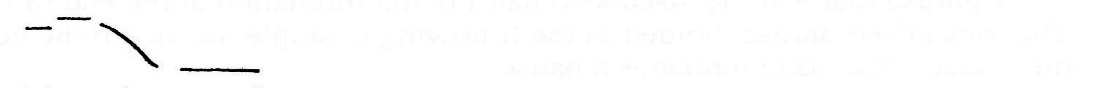
\includegraphics[width=\textwidth]{figures_mod/image22.jpeg}
\gll %
[\linieb{18}{iˈ}%
\linieb{20}{ki}%
\dline{20}{2}{24}{w-eka} %
\linieb{8}{jaaaa}] \\
go-\textsc{imp}.2p \textsc{intj}\\
\glt`Go, for heaven's sake!'
\z
}


 
\xbox{\textwidth}{
\ea%x912
\label{ex:2:x912}
% 
\includegraphics[width=\textwidth]{figures_mod/image23.jpeg}
\gll%
 [\dline{20}{2}{15}{se} 
 \linieb{14}{naːp} 
 \textstyleEmphasizedVernacularWords{
 \linieb{12}{ˈme}
 } %
 \dline{12}{3}{18}ma-e] \\
\textsc{intj} thus  not  say-\textsc{imp}.2s      \\
\glt`Goodness, don't say like that.'
\z
}

\subsection{Orthographic symbols}
%%\hypertarget{RefHeading18821935131865}


\tabref{tab:4:orthosymbols} shows the orthographic symbols for the phonemes. The semivowel /j/ is written as \textstyleStyleVernacularWordsItalic{y} due to the influence of Tok Pisin and English.  Because the orthography represents the phoneme inventory so closely, it is the orthographic symbols that are used in the vernacular examples throughout this thesis after the phonology chapter.


\begin{table}
\caption{Orthographic symbols for Mauwake phonemes}
\label{tab:4:orthosymbols}
\resizebox{\textwidth}{!}{\begin{tabular}{lcccccccccccccc}
\lsptoprule
Consonant phonemes & p & t & k & b & d & g & m & n & {\textphi} & s & l & r & w & j\\
Orthographic representation & p & t & k & b & d & g & m & n & f & s & l & r & w & y\\
\midrule
Vowel phonemes & i & e & a & o & u & \multicolumn{9}{l}{}\\
Orthographic representation & i & e & a & o & u & \multicolumn{9}{l}{}\\
\lspbottomrule
\end{tabular}}
\end{table}

\section{Syllables and phonotactics}\label{sec:2:2}
%%\hypertarget{RefHeading18841935131865}


\subsection{Syllable patterns}
%%\hypertarget{RefHeading18861935131865}


The syllable in Mauwake consists of one or two vowels forming the nucleus, with optional onset and/or coda of one consonant, \textsc{cv} being by far the most frequent syllable structure.\footnote{\citet[13]{Reesink1987} gives a short but good overview of syllable-final consonants in a number of \textsc{tng} languages.} The syllable patterns are given in \tabref{tab:2:syllablepatterns}.

\begin{table}
 \caption{Syllable patterns}
\label{tab:2:syllablepatterns}
\begin{tabular}{ll}
\mytoprule
\textsc{v}  &  \textsc{vc}\\
\textsc{cv} &  \textsc{cvc}\\
\textsc{vv} &  \textsc{vvc}\\
\textsc{cvv} & \textsc{cvvc} \\
\mybottomrule
\end{tabular}
\end{table}

Any vowel can fill the simple nucleus slot of the syllable. The complex nucleus slot is filled either by a geminate vowel or a diphthong. Diphthongs can occur in non-initial syllables too, but geminate vowels cannot. 

Any consonant can fill the onset slot, and all consonants except the voiced plosives, /{\textphi/} and /j/ can fill the coda slot of a syllable. The distribution of the voiced plosives and /{\textphi}/ is also restricted in that they very seldom occur later than in the second syllable of a word and, except for /j/, do not appear in inflectional morphology. \tabref{tab:5:consonantdistr} shows the possible distribution of consonants in a syllable.

\begin{table}
\caption{Consonant distribution in a syllable}
\label{tab:5:consonantdistr}
\setlength{\tabcolsep}{3pt}
\begin{tabular} {crclcccrcl}
\mytoprule
 &\textsc{c} & \textsc{v(v)} & \textsc{c} &&& & \textsc{c} & \textsc{v(v)} & \textsc{c}  \\
\midrule
p & + &    & + &&& n & + && +\\
t & + && + &&& {\textphi} & + && --\\
k & + && + &&& s & + && +\\
b & + && -- &&& l & + && +\\
d & + && -- &&& r & + && +\\
g & + && -- &&& w & + && +\\
m & + && + &&& j & + && --\\
\mybottomrule
\end{tabular}
\end{table} 


\subsection{Vowel sequences}
%\hypertarget{RefHeading18881935131865}

\tabref{tab:6:vowelseq} shows the possible two-vowel sequences in Mauwake. The only possible sequences beginning with either of the two mid vowels are geminate vowels; no other vowel sequences begin with a mid vowel. The other three vowels may combine with any vowel.


\begin{table}
\caption{Vowel sequences}
\label{tab:6:vowelseq}
\begin{tabular}{lllll}
\mytoprule 
ii &  & ai &  & ui\\
ie & ee & ae &  & ue\\
ia &  & aa &  & ua\\
io &  & ao & oo & uo\\
iu &  & au &  & uu\\
\mybottomrule
\end{tabular}
\end{table}

When the second vowel in a vowel sequence is articulatorily the same height or higher than the preceding vowel, the two form a diphthong, i.e., they are part of the same syllable \REF{ex:2:twovowel1}.

\ea
\label{ex:2:twovowel1}
\ea
/kae/  [\textipa{ˈkae}]  `my/our grandfather'
\ex
/kuina/  [\textipa{ˈkui.na}]  `woodborer'
\ex
/aowa/  [\textipa{ˈao.wa}]  `to tie around waist'
\z
\z


When the second vowel is lower than the first, the two vowels form the nuclei of two separate syllables \REF{ex:2:twovowel2}. 

\ea
\label{ex:2:twovowel2}
\ea
/sier/  [\textipa{s{\textsci}.ˈer}]  `husking stick'
\ex
/luaka/  [\textipa{l{\textupsilon}.ˈa.ka}]  `whitebait'
\ex
/kia/  [\textipa{k{\textsci}.ˈa}]  `white'
\z
\z


The high back vowel /u/ is considered lower than the high front vowel /i/, as it behaves similarly to the non-high vowels when following /i/ \REF{ex:2:twovowel3}.

\ea
\label{ex:2:twovowel3}
/niuk/  [\textipa{n{\textsci}.ˈuk}]  `let them give you'
\z

In an open syllable, all the diphthongs allowed by the language are possible. In a closed syllable, /ao/ is the only diphthong that has not been found; but it is very infrequent in an open syllable too. 

Sequences with three vowels are rare: /uau/ and /uai/ are the only ones I have found, and these only occur at morpheme breaks (marked with a hyphen in the examples), and there is a syllable break within the sequence as well \REF{ex:2:threevowels}.\footnote{A syllable break does not need to coincide with a morpheme break; in the examples above it does not.}  

\ea \label{ex:2:threevowels}
\ea
/kua-i-jem/    [\textipa{k{\textupsilon}.ˈai.jem}]      `I build'
\ex
/kua-uk/      [\textipa{k{\textupsilon}.ˈauk}]      `let them build'
\z
\z

\subsection{Consonant sequences} \label{sec:2.2.3}
%\hypertarget{RefHeading18901935131865}

No consonant sequences occur word-initially or -finally. In words with three or more syllables there are some word-medial clusters, which I believe to have resulted from vowel elision.  A vowel may be elided from a non-final syllable immediately following a stressed syllable, which is probably the least prominent syllable in the whole word.\footnote{According to \citet[11]{Sommerstein1977} this is a common process in languages.} It is mainly the high vowels that are dropped, since they are the least sonorant \REF{ex:2:vowelelision}. 

\ea
\label{ex:2:vowelelision}
\ea
/ikemika/  [\textipa{iˈkemka}]  `wound (nn)' 
\ex
/aakisa/  [\textipa{ˈaːksa}]  `now, today'
\ex
/pisikulaw/  [\textipa{piˈsiklaw}]  `grasshopper sp.'
\z
\z


A non-high vowel can also be elided if the adjacent stressed syllable has an identical vowel \REF{ex:2:vowelelisiontwo}:

\ea
\label{ex:2:vowelelisiontwo}
\ea
/kerekenam/  [\textipa{keˈreknam}]  `dollar bird'
\ex
/toonowaw/  [\textipa{ˈtoːnwaw}]  `honey eater'
\z
\z


Occasionally vowel elision takes place in a later syllable than that immediately following the stressed syllable \REF{ex:2:vowelelisionthree}: 

\ea
\label{ex:2:vowelelisionthree}
\ea
/o{\textphi}a{\textphi}ilika/  [\textipa{oˈ{\textphi}a{\textphi}ilka}]  `butterfly'
\ex
/aakuniwikin/  [\textipa{aːkuniwkin}]  `talk.2/3p.\textsc{ds}'
\z
\z

In some of these words the original vowel can still be perceived in slow pronunciation, but in others it has disappeared. Consequently, phonemic vowel clusters are currently developing in Mauwake,\footnote{The present orthography reflects this development in that consonant clusters are written especially 1) where the quality of the elided vowel cannot be established, and/or 2) when the elided form is in very frequent use.} and the distribution of \textsc{cvc} syllables is being extended to include word-medial position as well, and that of \textsc{vvc} and \textsc{cvvc} to include initial position in two-syllable words that have earlier had three syllables (\sectref{sec:2.3.2}).

No clear rules have been found for the site of the vowel elision, but some tendencies are as follows. Nouns have more elision than verb stems. A vowel is dropped much more often between non-homorganic than homorganic consonants. The voiceless velar plosive /k/ is the most frequent phoneme on either side of the elided vowel.

\section{Word}\label{sec:2.3}
%\hypertarget{RefHeading18921935131865}

\subsection{Defining a phonological word in Mauwake}
%\hypertarget{RefHeading18941935131865}

A phonological word is defined on the basis of a primary stress. Words are composed of one or more syllables. The number of syllables seldom exceeds ten, but compound words can be longer. A majority of the words have two or three syllables.  Every word has one syllable with a primary stress, and usually one or more unstressed syllables. 

In words of two or more syllables, the syllable containing the second vowel is stressed. Thus the first syllable is stressed if it contains a geminate vowel (\ref{ex:2:stressone}a) or a diphthong (\ref{ex:2:stressone}b). In all the other cases the second syllable is stressed (\ref{ex:2:stressone}c). When the stressed syllable is long, the stress falls equally on the whole vowel sequence (\ref{ex:2:stressone}d--e). 

\ea
\label{ex:2:stressone}
\ea
/aasa/  [\textipa{ˈaː.sa}]  `canoe'
\ex
/kuija/  [\textipa{ˈkui.ja}]  `it bites'
\ex
/a{\textphi}ura/  [\textipa{a.{ˈ}{\textphi}u.ra}]  `lime'
\ex
/siowa/  [\textipa{si.ˈo.wa}]  `dog'
\ex
/isaimija/  [\textipa{i.ˈsai.mi.ja}]  `(s)he heats (food)'
\z
\z

Both derivational and inflectional affixes may receive primary stress provided they are in a position where stress is normally placed \REF{ex:2:stresstwo}:

\ea
\label{ex:2:stresstwo}
\ea
  /aw-om-e/\\
  {}[\textipa{a.ˈwo.me}]  \\
weave-\textsc{ben}-\textsc{bnfy1}.\textsc{imp}.2s\\
\glt `weave it for me' 

\ex
  /um-o-k/ \\
 {}[\textipa{u.ˈmok}]  \\
die-\textsc{pa}-3s \\
\glt `(s)he died'
\z
\z



Clitics, on the other hand, never receive stress placement. Grammatically they are words, but phonologically they attach to the preceding word. If the preceding word is monosyllabic and has a short vowel, it still takes the primary stress when a clitic is added. The unmarked pronouns are a case in point: they retain their stress when clitics are added. Some non-phonemic lengthening takes place in the vowel of the pronoun stem \REF{ex:2:stressthree}.

\ea
\label{ex:2:stressthree}
\ea
/jo=ko/  [\textipa{ˈjo{\.{}.ko}}]  `\textit{I} (with neutral focus)'
\ex
/jos=ke/  [\textipa{ˈjo{\.{}s.ke}}]  `\textit{I} (and not someone else)' 
\z
\z

Compound words and some reduplicated words also have a secondary stress.  In the second (and third) compound of a compound word, that syllable has a secondary stress which in a single word would receive primary stress \REF{ex:2:stressfour}. 

\ea
\label{ex:2:stressfour}
\ea
/soomare-jiawem-ikemik/  [\textipa{ˈsoːmare-j{\textsci}{ˈ}{ˈ}awem-i{ˈ}{ˈ}kemik}]  `we were walking around'
\ex
/suuw-orom-ikua/  [\textipa{ˈsuːw-o{ˈ}{ˈ}rom-i{ˈ}{ˈ}kua}]  `he is pushing it down'
\z
\z

In those words where a long initial syllable is reduplicated as a whole, the second syllable is also long and receives a secondary stress \REF{ex:2:stressfive}:

\ea
\label{ex:2:stressfive}
\ea
/kui-kuisow/  [\textipa{ˈkui.{ˈ}{ˈ}kui.sow}]  `a few'
\ex
/suu-suusia/  [\textipa{ˈsuː.{ˈ}{ˈ}suː.sia}]  `thorny'
\z
\z

\subsection{Distribution of syllables in a word}\label{sec:2.3.2}
%\hypertarget{RefHeading18961935131865}

All syllable types except  \textsc{vc} can form a monosyllabic word. In polysyllabic words, the occurrence of a certain syllable type is determined by both its position in the word and the stress. 

\tabref{tab:7:syllabletypes} shows what syllable types occur in which positions in a word.  A blank space indicates that the syllable type does not occur in that particular word position at all, and parentheses indicate a rare occurrence. Double parentheses indicate new positions for closed syllables formed as a result of vowel elision (see \sectref{sec:2.2.3}). ``2nd'' indicates the second non-final syllable, and ``3rd-'' stands for the third or later non-final syllable in a polysyllabic word.


\begin{table}
\caption{Distribution of syllable types}
\label{tab:7:syllabletypes}
  \begin{tabular}{lcccccccccc}
  \mytoprule
  \multirow{2}{*}{\parbox{1cm}{Syllable\\type}} & \multicolumn{3}{c}{Stressed syllables} &  & \multicolumn{4}{c}{Unstressed syllables}  &  & \multirow{2}{*}{\parbox{1.2cm}{\mbox{The only} \mbox{syllable}}}\\
  & Initial & 2nd & Final &  & Initial & 2nd & 3rd- & Final &  & \\
  \midrule
  \textsc{v} &  & + & + &  & + &  & + & + &  & +\\
  \textsc{cv} &  & + & + &  & + & + & + & + &  & +\\
  \textsc{vv} & + & (+) & (+) &  &  &  & (+) & + &  & +\\
  \textsc{cvv} & + & + & (+) &  &  &  & + &  &  & +\\
  \textsc{vc} &  &  & + &  &  &  &  & + &  & \\
  \textsc{cvc} &  & ((+)) & + &  &  & ((+)) & ((+)) & + &  & +\\
  \textsc{vvc} & ((+)) &  & + &  &  &  &  & + &  & +\\
  \textsc{cvvc} & ((+)) &  & + &  &  &  &  & + &  & +\\
  \mybottomrule
  \end{tabular}
\end{table}

\footnotetext{`2nd' indicates the second non-final syllable, and `3rd-' stands for the third or later non-final syllable in a polysyllabic word.}


Some distributional characteristics can be summarised as follows.  The most frequent syllable type, \textsc{cv}, also has the widest distribution: a stressed initial syllable is the only position where it cannot occur, as an initial syllable with a single short vowel is always unstressed. The same reason accounts for the absence of \textsc{v} syllables in the same position. \textsc{v} syllables also never occur after a geminate vowel or diphthong, so they cannot occupy the second unstressed syllable position. A \textsc{vv} syllable in medial or final position is possible but very rare. The two previous statements may be combined to make the claim that there is some resistance towards \textsc{vvv} sequences in Mauwake. The syllables with a consonant coda only occur word finally, except where vowel elision has changed the syllable structure.  

\subsection{Morphophonology}\label{sec:2.3.3}
%\hypertarget{RefHeading18981935131865}

There are not many morphophonological alternations in Mauwake.  The most important is the rule system governing the vowel of the past tense suffix and the medial verb same-subject sequential action and simultaneous action suffixes (called the medial verb suffixes\footnote{There are also other medial verb suffixes, which are not  affected by these morphophonological rules.} in the discussion below).  Others include the change in the verbaliser suffix and the form of the completive aspect marker.

\subsubsection{Elision of word-final vowel}
%\hypertarget{RefHeading19001935131865}

The phoneme /a/ has a very high frequency as the word-final phoneme, particularly in the nouns and adjectives.  It accounts for approximately 85\% of all the vowel-final words.  In normal and fast speech this /a/ is often dropped from an unstressed word-final \textsc{cv} syllable, especially when followed by a word with an initial vowel. The elision rule is in  \REF{ex:2:elisionrule} and examples in \REF{ex:2:elisionexample}. 

\ea
\label{ex:2:elisionrule}
\begin{tabular}{c}\textsc{v}\\+central\\--stress\\    \end{tabular}
\begin{tabular}{c}    $\rightarrow $ {\O}  /  \textsc{c} \_\_  \#  \textsc{v} \\~\\~\\    \end{tabular}
\z

\ea
\label{ex:2:elisionexample}
\ea
/koora unowa/  [\textipa{ˈkoːr  u{ˈ}nowa}]  `many houses'
\ex
/takira {\textphi}aara/  [\textipa{taˈkir  {ˈ}{\textphi}aːra}]  `boys' house'
\ex
/siiwa eliwa/  [\textipa{ˈsiːw  e{ˈ}liva}]  `good/bright moon'
\ex
/ikoka uura/  [\textipa{iˈkok  {ˈ}uːra}]  `later at night'
\z
\z

In some cases even a stressed /a/ is elided, and the stress moves to the following vowel in the utterance.  This mainly happens with the accusative pronouns, which tend towards cliticization \REF{ex:2:stressedelision} (\sectref{sec:3.5.3}).

\ea
\label{ex:2:stressedelision}
/me ne{\textphi}a uru{\textphi}am/  [\textipa{ˈme ne{\textphi} {ˈuru}{\textphi}am}]  `I didn't see you'
\z

In compound words the final /a/ is dropped from the first constituent even when the second begins with a consonant, except when the final syllable of the first constituent is stressed \REF{ex:2:compoundelision}.  

\ea
\label{ex:2:compoundelision}
\ea
/aara muuka/  [\textipa{ˈaːr {ˈ}muːka}]  `chick'
\ex
/emera tapaka/  [\textipa{eˈmer ta{ˈ}paka}]  `sago cake'
\ex
/mera soo/  [\textipa{meˈra {ˈ}soː}]  `fish trap'
\z
\z

\subsubsection{Reduplication}\label{sec:2.3.3.2}
%\hypertarget{RefHeading19021935131865}

There are various patterns of reduplication in Mauwake. With a few exceptions, reduplication takes place at the beginning of the word.  The meaning involves plurality in one way or another; with verbs it indicates repeated action and/or the object of the action ending up in several pieces. Occasionally with adjectives it also indicates enhanced quality (\sectref{sec:3.3}).

How a word is reduplicated can to some extent be predicted from the phonological shape of the word.  Type 1 below is the most common, 2 and 3 are the only possible ones for the words with a short and a long initial vowel respectively.  Reduplication process does not always respect syllable boundaries.

\paragraph[Type 1]{Type 1}
%\hypertarget{RefHeading19041935131865}

Everything up to and including the first vowel of the stressed syllable is reduplicated.  Even with the reduplication these words retain the normal stress pattern: the second syllable of the reduplicated form is stressed, because regardless of whether one or two syllables are reduplicated the first syllable in this type is always short. When two of syllables are reduplicated, the originally stressed syllable of the word root gets a secondary stress \REF{ex:2:reduptypeone}.

\ea
\label{ex:2:reduptypeone}
\ea
/pu-puukija/  [\textipa{pu.ˈpuː.ki.ja}]  `cut into pieces'
\ex
/pu-puija/  [\textipa{pu.ˈpui.ja}]  `break into pieces'
\ex
/pere-perekija/  [\textipa{pe.ˈre.pe.{ˈ}{ˈ}re.ki.ja}]  `tear into pieces'
\ex
/kiri-kiripija/  [\textipa{ki.ˈri.ki.{ˈ}{ˈ}ri.pi.ja}]  `turn round \& round, mix'
\ex
/mane-maneka/  [\textipa{ma.ˈne.ma.{ˈ}{ˈ}ne.ka}]  `(many) big (things)'
\z
\z


\paragraph{Type 2:  \textsc{v}\textsubscript{1}\textsc{c}\textsubscript{1}\textsc{v}\textsubscript{1} - \textsc{v}\textsubscript{1}\textsc{c}\textsubscript{1}\textsc{v}\textsubscript{2}\textsc{c}\textsubscript{2}\textsc{v}(\textsc{v}\textsubscript{3})\textsc{x}}
%\hypertarget{RefHeading19061935131865}

In the words of the second type, the reduplication repeats the initial vowel and consonant of the word root, adding another vowel of the same quality after the consonant.  In these words the stress shifts from the second syllable of the root to the final vowel of the reduplicated element.  Phonetically this vowel usually merges into one with the following vowel, which always has the same quality \REF{ex:2:reduptypetwo}.  Stresswise this creates an interesting pattern, where a syllable with a primary stress is followed by one with secondary stress.  Types 3 and 4 also have this kind of stress pattern.

\ea
\label{ex:2:reduptypetwo}
\ea
/ele-eliwa/  [\textipa{e.ˈle.{ˈ}{ˈ}li.wa}]  `(many) good (things)'
\ex
/ara-arow/  [\textipa{a.ˈra.{ˈ}{ˈ}row}]  `in threes'
\ex
/oko-okaiwi/  [\textipa{o.ˈko.{ˈ}{ˈ}kai.wi}]  `this side and that'
\z
\z

\paragraph{Type 3:  \textsc{v}\textsubscript{1}\textsc{v}\textsubscript{1}\textsc{c}\textsubscript{1} - \textsc{v}\textsubscript{1}\textsc{v}\textsubscript{1}\textsc{c}\textsubscript{1}\textsc{v}\textsubscript{2}\textsc{x}}
%\hypertarget{RefHeading19081935131865}

A very small group of words has this type of reduplication, where the initial geminate vowel and the following consonant are reduplicated.  The result is a word where both the first and the second syllable have a complex nucleus, a word type not allowed in the simple non-reduplicated words.  In these reduplicated words the first syllable receives primary stress and the second syllable secondary stress.  The first syllable has a syllable pattern (\textsc{vvc}) which is not possible for the first syllable in a non-reduplicated polysyllabic word \REF{ex:2:reduptypethree}.

\ea
\label{ex:2:reduptypethree}
\ea
/iiw-iiwa/  [\textipa{ˈiːv.{ˈ}{ˈ} iː.va}]  `(many) short (things)'
\ex
/iin-iinan/  [\textipa{ˈiːn.{ˈ}{ˈ} iː.nan}]  `(the things) high up'
\z
\z

\paragraph{Type 4:  \textsc{c}\textsubscript{1}\textsc{v}\textsubscript{1}\textsc{v}\textsubscript{2} - \textsc{c}\textsubscript{1}\textsc{v}\textsubscript{1}\textsc{v}\textsubscript{2}\textsc{x}}
%\hypertarget{RefHeading19101935131865}

In this type the long first syllable is repeated entirely, but nothing else.  The two vowels in the initial syllable may be identical or different in quality \REF{ex:2:reduptypefour}. This is not a very common pattern.

\ea
\label{ex:2:reduptypefour}
\ea
/kui-kuisow/  [\textipa{ˈkui.{ˈ}{ˈ}kui.sow}]  `a few'
\ex
/soo-soomarija/  [\textipa{ˈsoː.{ˈ}{ˈ}soː.ma.ri.ja}]  `amble, stroll'
\z
\z

\paragraph{Unusual reduplications}
%\hypertarget{RefHeading19121935131865}

The word \textstyleStyleVernacularWordsItalic{gelemuta} `small' has two unusual reduplicated forms, where the end of the word is changed: \textstyleStyleVernacularWordsItalic{gelemutitik} and \textstyleStyleVernacularWordsItalic{gelemutumut} `(many) small (things)'.  Type 1 reduplication rule can also be applied to these already reduplicated forms, although not to the root \REF{ex:2:redupgelemuta}.

\ea
\label{ex:2:redupgelemuta}
\ea
/gele-gelemutitik/  [\textipa{ge.ˈle.ge.{ˈ}{ˈ}le.mu.ti.tik}]  `very small (pl.)'
\ex
*/gele-gelemuta/
\z
\z

The verb \textstyleStyleVernacularWordsItalic{wafuriya} `throw' also has an irregular reduplicated form: only the second syllable is reduplicated \REF{ex:2:redupwafuriya}.

\ea
\label{ex:2:redupwafuriya}
/wa{\textphi}u{\textphi}urija/  [\textipa{va.ˈ{\textphi}u.{\textphi}u.ri.ja}]  `throw around'
\z

The reduplication for the word \textstyleStyleVernacularWordsItalic{owowa} `village' occurs at the beginning of the word, but it does not follow any of the patterns above \REF{ex:2:redupowowa}. So far it is the only one of its kind found.

\ea
\label{ex:2:redupowowa}
/owow-owowa/  [\textipa{o.ˈwo.wo{ˈ}{ˈ}wo.wa}]  `(many/all) villages'
\z

Mauwake has a number of nouns of the following the pattern \textsc{c}\textsubscript{1}\textsc{v}\textsubscript{1}\textsc{c}\textsubscript{2}\textsc{v}\textsubscript{2} \textsc{c}\textsubscript{1}\textsc{v}\textsubscript{1}\textsc{c}\textsubscript{2} , which looks like reduplication, but with the word-final vowel deleted.  However, these words do not have any semantic relationship with a corresponding \textsc{c}\textsubscript{1}\textsc{v}\textsubscript{1}\textsc{c}\textsubscript{2}\textsc{v}\textsubscript{2} word in cases where the latter may exist.  Words of this type are not considered to have resulted from reduplication \REF{ex:2:nonredup}.

\ea
\label{ex:2:nonredup}
\ea
/mulamul/  [\textipa{muˈlamul}]  `trevally'
\ex
/jawejaw/  [\textipa{jaˈvejav}]  `hunting magic'
\z
\z

Similarly, words of the pattern \textsc{c}\textsubscript{1}\textsc{v}\textsubscript{1}\textsc{c}\textsubscript{1}\textsc{v}\textsubscript{1}\textsc{c}\textsubscript{2}\textsc{v}\textsubscript{2} are not considered reduplicated forms \REF{ex:2:nonredup2}.  Firstly, there is no semantic relationship with a corresponding \textsc{c}\textsubscript{1}\textsc{v}\textsubscript{1}\textsc{c}\textsubscript{2}\textsc{v}\textsubscript{2} word, even if the latter exists. Secondly, in Mauwake there is a very strong tendency to have the same vowel in the first two syllables of trisyllabic or longer words, whether the consonant is the same or not. 

\ea
\label{ex:2:nonredup2}
\ea
/momora/  [\textipa{moˈmo.ra}]  `fool(ish)'
\ex
/sisina/  [\textipa{siˈsi.na}]  `edge'
\z
\z

\subsubsection{Past tense and medial verb suffixes}\label{sec:2.3.3.3}
%\hypertarget{RefHeading19141935131865}


There are three past tense verb suffixes for second and third person singular forms, -\textstyleStyleVernacularWordsItalic{a}, -\textstyleStyleVernacularWordsItalic{e} and -\textstyleStyleVernacularWordsItalic{o}.  Which one is chosen for which verb is determined mainly by the phonemes in the stem final syllable.\footnote{Most of these rules were originally worked out by Kwan Poh San.}

The two basic allomorphs for the past tense suffix are \{-a\} and \{-\textsc{e}\}. /\textstyleStyleVernacularWordsItalic{-}o/ is a subgroup of the allomorph \{-\textsc{e}\}. The subgrouping is based on the fact that the \textstyleStyleVernacularWordsItalic{-a/}\textstyleStyleVernacularWordsItalic{-e} distinction runs through the whole past tense paradigms and occurs in the medial verb suffixes as well, whereas the \textstyleStyleVernacularWordsItalic{-}\textstyleStyleVernacularWordsItalic{e/-o} distinction only occurs in the second and third person past tense forms of some verbs.  According to the rounding rule below \REF{ex:2:pasttenseruleEo}, \{-\textsc{e}\} is realized as /-o/ when both following a [+ labial] phoneme (either a labial consonant or the high rounded vowel /u/) and preceding a non-labial consonant \REF{ex:2:Eoex}. 

\ea
\label{ex:2:pasttenseruleEo}
\{\textsc{e}\} {{\textgreater}} /o/  /  \textsc{x} \textsubscript{\textsc{lab}}  \_\_  \textsc{c}\textsubscript{\textsc{non-lab}} 
\z

\ea
\label{ex:2:Eoex}
\ea
/aaw-o-k/  `(s)he got (it)'  cf.  /aaw-e-m/  `I got (it)'
\ex
/mu-o-n/  `you swallowed'  cf.  /mu-e-m/  `I swallowed'
\z
\z

The discussion below only mentions the past tense suffixes. The vowels in the  the medial verb suffixes are the same but do not have the allophonic variation between /-e/ and /-o/.  

The morphophonological rules governing the choice of past tense suffixes are listed in their order of relative strength, with regard to the number of cases in the data\footnote{The count included 273 verbs with the past tense suffix {\nobreakdash-\textstyleStyleVernacularWordsItalic{a}},  364 with the suffix -\textstyleStyleVernacularWordsItalic{e}.} as well as the number of exceptions.

\ea
\textstyleEmphasizedWords{{Rule 1}}.  With a stem-final high vowel /i/ or /u/, the past tense suffix is always \{\nobreakdash-\textsc{e}\} \REF{ex:2:rule1ex}.
\z


\ea
\label{ex:2:rule1ex}
\ea
/waki-\textstyleEmphasizedVernacularWords{e}-k/  `(s)he fell down'
\ex
/nepi-\textstyleEmphasizedVernacularWords{e}-k/  `(s)he raised animals'
\ex
/mu-\textstyleEmphasizedVernacularWords{o}-k/  `(s)he swallowed'
\ex
/karu-\textstyleEmphasizedVernacularWords{o}-k/  `(s)he ran'
\z
\z

\ea
\textstyleEmphasizedWords{{Rule 2}}.  With a stem-final alveolar nasal /n/, the suffix is nearly always /-e/ \REF{ex:2:rule2ex}.
\z

\ea
\label{ex:2:rule2ex}
\ea
/kekan-\textstyleEmphasizedVernacularWords{e}-k/  `it hardened'
\ex
/peren-\textstyleEmphasizedVernacularWords{e}-k/  `it tore'
\ex
/riirin-\textstyleEmphasizedVernacularWords{e}-k/  `(s)he laughed'
\ex
/solon-\textstyleEmphasizedVernacularWords{e}-k/  `it glided'
\ex
/uuwun-\textstyleEmphasizedVernacularWords{e}-k/  `(s)he chatted'
\z
\z

In the data there are 128 verb stems ending in /n/, and only 15 take the suffix \{\nobreakdash-a\}. In some cases there is a conflict between rules 2 and 3 (below), and 13 of those exceptions follow Rule 3.

\ea
\textstyleEmphasizedWords{{Rule 3.} } When the stem final syllable has a low vowel, there is dissimilation between the vowels in the stem final syllable and the past tense suffix. For these morphophonological rules the mid vowels are also considered low, so that there is height distinction only between high and low vowels.
\z

\ea
\begin{tabular}{c}X \\~ \\~ \end{tabular}
\begin{tabular}{c}V \\ +low\\{\textalpha} central \end{tabular}
\begin{tabular}{c}(C) \\~ \\~ \end{tabular}
\begin{tabular}{c}+ \\~ \\~ \end{tabular}
\begin{tabular}{c}\textbf{V} \\ +low\\-{\textalpha} central \end{tabular}
\z

The past tense suffix tends to be \{-a\}, when the last vowel in the stem is /e/ or /o/ \REF{ex:2:rule3ex}. 

\ea
\label{ex:2:rule3ex}
\ea
/aner-\textstyleEmphasizedVernacularWords{a}-k/  `(s)he aimed at'
\ex
/sirek-\textstyleEmphasizedVernacularWords{a}-k/  `it scratched'
\ex
/imen-\textstyleEmphasizedVernacularWords{a}-k/  `(s)he found
\ex
/on-\textstyleEmphasizedVernacularWords{a}-k/  `(s)he did/made'
\ex
/soop-\textstyleEmphasizedVernacularWords{a}-k/  `(s)he buried'
\z
\z

In words with /a/ as the last vowel in the stem, the past tense suffix tends to be \{\nobreakdash-\textsc{e}\} \REF{ex:2:rule3exx}.\footnote{In the data there are 187 verbs that follow this rule and 19 that do not.}

\ea
\label{ex:2:rule3exx}
\ea
/serak-\textstyleEmphasizedVernacularWords{e}-k/  `(s)he wiped'
\ex
/war-\textstyleEmphasizedVernacularWords{e}-k/  `(s)he killed it'
\ex
/ma-\textstyleEmphasizedVernacularWords{e}-k/  `(s)he said'
\ex
/ekap-\textstyleEmphasizedVernacularWords{o}-k/  `(s)he came'
\ex
/aaw-\textstyleEmphasizedVernacularWords{o}-k/  `(s)he got/took'
\z
\z

\ea
\textstyleEmphasizedWords{{Rule 4}}. When a high vowel is followed by a stem-final consonant /k/, /t/, /s/, /r/ or /l/, the past tense suffix is \{-a\}.  This group of consonants includes nearly all of the non-labial consonant phonemes; /n/ is handled in Rule 2, the voiced stops never occur stem-finally and /j/ hardly ever does \REF{ex:2:rule4ex}.  
\z

\ea
\label{ex:2:rule4ex}
\ea
/puuk-\textstyleEmphasizedVernacularWords{a}-k/  `(s)he cut'
\ex
/mik-\textstyleEmphasizedVernacularWords{a}-k/  `(s)he speared'
\ex
/itit-\textstyleEmphasizedVernacularWords{a}-k/  `(s)he smashed'
\ex
/anetir-\textstyleEmphasizedVernacularWords{a}-k/  `(s)he tied'
\ex
/{\textphi}uur-\textstyleEmphasizedVernacularWords{a}-k/  `(s)he blew'
\ex
/a{\textphi}ilil-\textstyleEmphasizedVernacularWords{a}-k/  `it was sweet'
\z
\z

With the rest of the verbs, i.e. total of about 25\% of all the basic verbs, it is very difficult to find any rules governing the choice of the past tense suffix \REF{ex:2:norule}.

\ea
\label{ex:2:norule}
\ea
/tiim-\textstyleEmphasizedVernacularWords{a}-k/  `(s)he touched'
\ex
/aru{\textphi}-\textstyleEmphasizedVernacularWords{a}-k/  `(s)he hit'
\ex
/oosip-\textstyleEmphasizedVernacularWords{o}-k/   `(s)he sweated'
\ex
/{\textphi}iririm-\textstyleEmphasizedVernacularWords{o}-k/  `(s)he squeezed'
\ex
/u{\textphi}-\textstyleEmphasizedVernacularWords{o}-k/  `(s)he danced'
\ex
/iw-\textstyleEmphasizedVernacularWords{o}-k/  `(s)he gave him/her'
\z
\z

A few verbs apparently have dropped the past tense suffix altogether.  Most of these have the stem ending in the vowel sequence /ua/ \REF{ex:2:nopasttensesuffix}:

\ea
\label{ex:2:nopasttensesuffix}
\ea
/kua-{\O-k}/  `he built'
\ex
/wua-{\O-k}/  `(s)he put'
\ex
/piipua-{\O-k}/  `(s)he left'
\z
\z

Another verb where the past tense suffix vowel seems to have disappeared is /oro-{\O}-k/ `(s)he went down'.  If the second vowel were to be taken as the suffix this verb would defy the basic rules, since the vowel /o/ is retained right through the past tense paradigm, and with the root vowel /o/ the suffix should be \{-a\}.  Positing /oro-/ as the root solves the question why the present tense form is /ora-/: since /oi/ is not a permitted vowel sequence on Mauwake, the low back vowel /o/ has changed into the low central vowel /a/ when preceding the high front vowel /i/ of the present tense suffix.

The verbs in the Mauwake dictionary are marked as belonging to Class 1 or Class 2, the former taking \{-a\} and the latter \{-\textsc{e}\} as the past tense suffix. This is because of the following reasons: 1) the rules are rather complicated, 2) there are a number of exceptions to the main rules, and 3) there are pairs of homophonous verb roots that take a different past tense suffix each \REF{ex:2:homophonousroots}.

\ea
\label{ex:2:homophonousroots}
\ea
/iw-\textstyleEmphasizedVernacularWords{a}-k/  `(s)he went'
\ex
/iw-\textstyleEmphasizedVernacularWords{o}-k/  `(s)he gave him/her'
\ex
/miim-\textstyleEmphasizedVernacularWords{a}-k/  `(s)he heard'
\ex
/miim-\textstyleEmphasizedVernacularWords{o}-k/  `(s)he preceded'
\ex
/op-\textstyleEmphasizedVernacularWords{a}-k/  `(s)he held'
\ex
/op-\textstyleEmphasizedVernacularWords{o}-k/  `it boiled'
\ex
/keen-\textstyleEmphasizedVernacularWords{a}-k/  `it touched'
\ex
/keen-\textstyleEmphasizedVernacularWords{e}-k/  `it was hot'
\z
\z

\subsubsection{Inchoative suffix} \label{sec:2.3.3.4}
%\hypertarget{RefHeading19161935131865}

The verbalizer for both adjectives and nouns is the inchoative suffix \{-a\textsc{r}\}, the root of the verb `to become' (\sectref{sec:3.8.2.2.2}).  In most environments it is realized as /\nobreakdash-ar/, but becomes /-al/ when the last syllable of the root contains the lateral consonant /l/ \REF{ex:2:inchoative}.  An illustrative example is the word \textstyleStyleVernacularWordsItalic{samora/damola} `bad', which takes a different verbalizer depending on the root allomorph.

\ea
\label{ex:2:inchoative}
\ea
/supuk\textstyleEmphasizedVernacularWords{-ar}-e-k/  `it got wet' 
\ex
/duduw-\textstyleEmphasizedVernacularWords{ar}-e-k/  `it became blunt'
\ex
/samor-\textstyleEmphasizedVernacularWords{ar}-e-k/  `it broke/spoiled'
\ex
/damol-\textstyleEmphasizedVernacularWords{al}-e-k/  `it broke/spoiled'
\ex
/memel-\textstyleEmphasizedVernacularWords{al}-e-k/  `it became tame'
\ex
/masi-\textstyleEmphasizedVernacularWords{al}-e-k/  `it became bitter'
\z
\z

In a few cases the inchoative suffix has the form /-al/ although there is no lateral consonant in the root.  This might be expected, since there is some fluctuation between the liquids /l/ and /r/ in Mauwake: /eliwa/ {\Tilde} /eriwa/ `good', /samora/ {\Tilde} /damola/ `bad'.\footnote{In Trans New Guinea, as well as other Papuan, languages it is also very common to have only one liquid, with /l/ and /r/ as allophones of the same phoneme (\citealt[55]{Wurm1982}, \citealt[55]{Foley1986}).} 


\subsubsection{Completive aspect marker}
%\hypertarget{RefHeading19181935131865}

The completive aspect marker (\sectref{sec:3.8.5.1.1.1}) has its origin in the verb for `put', \textstyleStyleVernacularWordsItalic{wua}\nobreakdash-,\footnote{The verb `put' is commonly used as a completive aspect marker in Papuan languages (\sectref{sec:3.8.5.1.1.1}).} but this connection has by now become opaque and the speakers consider it a morpheme on its own, \textstyleStyleVernacularWordsItalic{pu}- \REF{ex:2:completive}.  The initial /p/ results from assimilation with the final /p/ of the same-subject sequential action medial verb form obligatorily preceding the completive morpheme.

\ea
\label{ex:2:completive}
\gll\itshape en-ep  \itshape wu-a-k  {\upshape \textgreater}  \itshape enep-pu-a-k \\ 
eat-\textsc{ss}.\textsc{seq}  put-\textsc{pa}-3s  {{\textgreater}}  eat-\textsc{ss}.\textsc{seq}-\textsc{cmpl}-\textsc{pa}-3s\\
\glt `(s)he ate'
\z

\subsection{Loan words}
%\hypertarget{RefHeading19201935131865}

When words are borrowed from other languages, they are usually made to conform to the Mauwake phonology, if they do not originally do so.  Thus Tok Pisin \textstyleForeignWords{kikim} `kick' becomes \textit{kiikim}- in Mauwake; the word retains the original Tok Pisin word-initial stress, and the vowel in the first syllable becomes a geminate.  The initial glottal fricative /h/ in the original becomes a lengthened vowel in Mauwake, e.g. Tok Pisin \textstyleForeignWords{handet} `hundred' changes into \textstyleStyleVernacularWordsItalic{aandet}  in Mauwake.

The only non-native phoneme regularly retained in the loan word is the velar nasal /{\ng}/, particularly prominent in the neighbouring language, Mala, and also used in personal names \REF{ex:2:Malaloan}:

\ea
\label{ex:2:Malaloan}
/nadi{\ng-ar-e-k/}  `(s)he decorated him/herself'
\z

Since consonant sequences are quite rare in Mauwake, loan words with consonant clusters tend to have vowels inserted between the consonants.  With the ever-growing influence of Tok Pisin, vowel insertion is getting less common.  A combination of a nasal plus a homorganic stop is always retained in a loan word (\tabref{tab:2:loanwords}).

\begin{table} 
 \caption{Loanwords with a combination of nasal plus homorganic stop.}
\label{tab:2:loanwords}
\begin{tabular}{>{\itshape}l>{\itshape}l>{\itshape}l}
\mytoprule
\upshape Tok Pisin   & \upshape Mauwake  & \upshape English\\
\midrule 
glas & galas&  glass \\
{trinde}&  tirinde &  Wednesday \\
{namba} & naamba & number \\
{handet} & aandet & hundred \\
\mybottomrule
\end{tabular}

\end{table}


\renewcommand{\exfont}{\itshape}
\renewcommand{\eachwordone}{\itshape}